\documentclass[conference]{IEEEtran}
\IEEEoverridecommandlockouts
\usepackage{url} 
\usepackage{cite}
\usepackage{amsmath,amssymb,amsfonts}
\usepackage{algorithmic}
\usepackage{graphicx}
\usepackage{textcomp}
\usepackage{xcolor}
\def\BibTeX{{\rm B\kern-.05em{\sc i\kern-.025em b}\kern-.08em
    T\kern-.1667em\lower.7ex\hbox{E}\kern-.125emX}}

\begin{document}

\title{Temporal Evolution In Commit Size Distribution\\
  \thanks{----} }

\author{\IEEEauthorblockN{-} \IEEEauthorblockA{-} \and
  \IEEEauthorblockN{-} \IEEEauthorblockA{-} }

\maketitle

\begin{abstract}
  Software nowadays is almost exclusively developed using source
  control systems. Traditionally, the study of the evolution of this
  type of systems is usually done from the perspective of
  self-organized complex systems, since the version-control tools used
  allow a community-oriented development without a fixed or appointed
  leader. Understanding if and how a software development team
  self-organizes might give hints on how to improve productivity,
  reduce bugs or, in the case of open source systems based on
  volunteer woor, reduce churn and increase engagement.

  However, one of the essential characteristics needed to understand
  this type of systems' behaviour and to know if we are truly dealing
  with an auto-organized community is the appearance or not of a power
  law in the events' size distributions.  In this case, we have chosen
  to treat commits as our events, that is, additions to the code by
  users.
  % - This is our choice and should be presented that way. Other
  % people might use a different thing, like file size, author
  % interactions or whatever - JJ

  But we have to be extremely cautious with this kind of approach,
  because the existence or not of this type of distributions should be
  always analyzed mathematically to minimize posible sources of bias.
  We will use the concept of hypothesis tests for that purpose, that
  is, checking what is the likelihood that our data follows a power
  law distribution instead of some other with similar characteristics.

  The conclusions of these tests may not shed light on whether we are
  in a state of self-organization.  Software development is a process
  that evolves over time and analysis at a specific moment is not
  significant.  Our approach in this work uses a temporal analysis
  over the evolution of commit's distribution in software
  projects. For that, we have selected a set of repositories that
  exhibit singular behaviors such as a large number of contributions
  versus few or inconclusive results in statistical tests.

  Our study seeks to provide conclusive evidence about the state of
  the chosen repositories, answering wether they have not reached a
  state of self-organization in all its evolution (that is, never
  present power law distributions) or, if they have done so, but due
  to other code insertions and to the temporary nature of the creative
  process, this self-organized state has been altered.

  

\end{abstract}

\begin{IEEEkeywords}
  Complex systems, self-organizing systems, self-organized
  criticality, power laws, software development, software repositories
\end{IEEEkeywords}


%%%%%%%%%%%%%%%%%%%%%%%%%%%%%%% INTRODUCTION %%%%%%%%%%%%%%%%%%%%%%%%%%%%%%%
\section{Introduction}\label{introduction}


% --------------------------------------------------------


\section{State of the art}\label{soa}



% --------------------------------------------------------


\section{Methodology}
\label{sec:method}

In this section we are going to explain the methods used in our
research.

Our methodology hinges on four distinguished parts of our workflow.
First of all, we highlight the process of data extraction, which
follows particular considerations within the usual study of
repositories. Later we talk about the mathematics behind our
approaches to understand the distribution behind the data, which leads
to the third part, where we collect the information obtained in the
previous one and explain how it has been classified. Finally we added
a section of visualization to briefly explain some changes that can be
disconcerting when it comes to visualizing possible power laws.


\subsection{Data extraction and division}
%% rewrite
We have chosen 5 repositories in different states of development.
These repositories were chosen in \cite{Merelo2016:repomining}, for
several reasons: They all represent a wide array of languages and
functionalities, from web frameworks such as Django to Atom plugins,
through one-of-a-kind frameworks such as Docker.

Normally a code repository is related to a software project, for this
reason, it is usual that they include several different languages
which are used in different parts of the project.  This mixture of
languages also offer a big range of variability between languages that
are interpreted or compiled, either to machine code or to bytecode.

Repositories vary also in {\em professionalism}, that is, the team
behind that software project. From a small Atom editor plugin to
TensorFlow, an open library created and maintained by a fully
professional community.

Repository mining was done during the months of January to March 2017,
with the second sweep of the same repositories performed in February
2019.

The way we look at changes in the repository was initially proposed by
\cite{Merelo2016:repomining} and was also used in
\cite{merelo2017self}, where a deeper explanation can be found.


This procedure is based on three main concepts:
\begin{itemize}
\item The usage of a discrete timeline formed by the commits, with
  every commit counting as time=1.
\item Work with selected files in the repository, excluding those
  related to images or style
\item We take the largest value from the inserted and deleted lines of
  code.
\end{itemize}

%% New
Since we want to understand how commits distribution evolve, we
decided to divided each dataset into 5 different sections, each of
them of equal size. These division are made in the commit order and
represent progressive temporal windows in a evolving system like these
repositories.

With those divisions made we generate 5 different datasets, each one
contains its corresponding section and all the previous ones, which
means we analyze all the information until the final commit of the
section.  These hopefully provide us a sigth in the evolution in time
of the commits distribution.


\subsection{Hypothesis tests}

Once those datasets are extracted, we begin to check the probability
of finding powerlaw or similar heavy-tailed distributions in the
dataset.

First of all we could test that checks whether the observed data set
actually follows a power-law, instead of only visualize the result.
This kind of tests can vary based on different measured and
techniques. The most popular one is presented in
\cite{clauset2009power}, which consists in using a goodness-of-fit
hypothesis test via bootstrapping procedure.


Up to this point, we have detected what data sets are unlikely to be
fitted by a power law in any of its range. Notice, on the contrary
case, that we are only assuming that we can not discard that a power
law is generating the data.  However, as there is some probability of
the appearance of this distribution in our data we can study and
analyze how its two main parameters may evolve between 2017 and 2019.

As it is unrealistic to think that a power law distribution will fit
all our data, our first step is to check what portion of the data
could be fitted with a power law, or in other words, what is the
minimal value (if there is one) from which the scaling relationship of
the power law begins \footnote{This is a fair assumption since we are
  working with heavy-tailed distributions and our main interest is the
  behaviour of the tail of our data.}.  This value is usually noted by
$x_{min}$ and is our first parameter.

Once we have the first value, we proceed to estimate the scale of our
power law.  As it is shown in papers like \cite{newman2005power,
  clauset2009power}, least square method is a poor but wide-spreaded
way to proceed when estimating the scale parameter. Instead, we are
going to use a direct method describe in \cite{clauset2009power} and
implemented in \cite{alstott2014powerlaw} that use the data values we
have. This method is known to produce a very nice fit with less error
than the others mentioned above.

Up to this point we have revisited our way of analyze power law
fitting and the estimation of our parameters. However, there is a more
deep question unanswered: does our data really follow (in a
statistically relevant way) a power law?  This kind of answers were
lacking in \cite{merelo2017self} and they are relevant independently
our first test's results, since they usually offer an unbiased look of
the data .

Taking into account that our main question is wether a power law is
the best description of our data, we choose to apply a comparative
test that could evaluate if there are any alternative distribution
that could have generated our data with greater likelihood than a
power law. That is the main reason why we choose to use a
log-likelihood ratio test implemented in \cite{alstott2014powerlaw}.
There are two algorithm's outcomes. First we have the log-likelihood
ratio between the two candidate distributions. The sign of this
quantity will point out which distribution is more likely to be
producing out data. After it, we calculate the signification of this
ratio, a P-value. Following \cite{alstott2014powerlaw} indications we
establish our P-value threshold at $p=0.05$; above that point the
loglikehood ratio has no significance and we can not decide which
distribution is better fitting out data.

\subsection{Classification}

Since we are trying to uncover any variation we have decide to
summarize all the tests in a single statement, and see if it
changes. We use the scale proposed in \cite{clauset2009power}, which
is described as:
\begin{itemize}
\item \textbf{None}: Data-set is probably not distributed by a power
  law (first test failed).
\item \textbf{Moderate}: Power law is a possible fit but there are
  other plausible distributions that fit the data.
\item \textbf{Good}: Power law is a possible fit and none of the other
  distributions is plausible.
\item \textbf{Truncated}: when truncated power law is clearly favored
  over a simple power law
\end{itemize}

A relevant remark should be made: These scale clearly can obscure out
conclusions.  Maybe a more refined scale can expose slightly smaller
changes and split two equal classification (made with the scale
presented ) in two different categories.

\subsection{Visualization}
 
For the graphics included we should specify that we are going to use
the probability density function (PDF) in our plots. Due to the
requirement of binning the data to this type of graphic, we are going
to use a logarithmic spacing, since it reduces the statistical errors
in the tail in log-log plots at it is stated in
\cite{newman2005power}.



% --------------------------------------------------------


\section{Results}
\label{res}

\begin{figure*}[htbp]
	\centerline{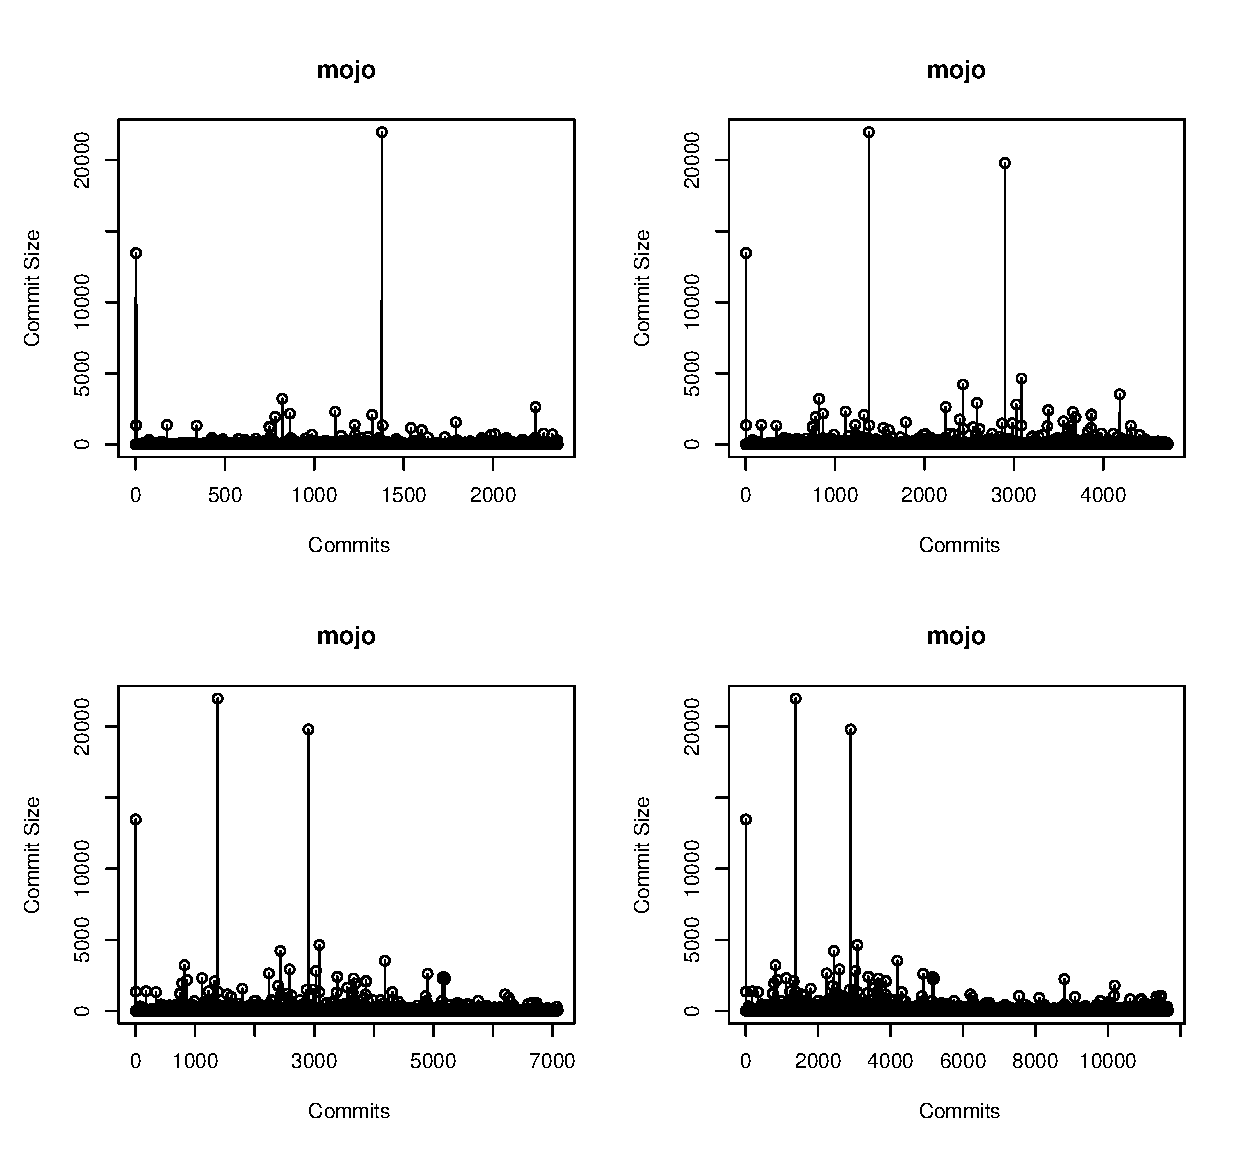
\includegraphics[width=0.95\textwidth]{img/mojo_temporal.eps}}
	\caption{Evolution in temporal windows of Commit size vs. Commit number in mojo's repository.}
	\label{fig:cask}
      \end{figure*}

\begin{figure*}[htbp]
	\centerline{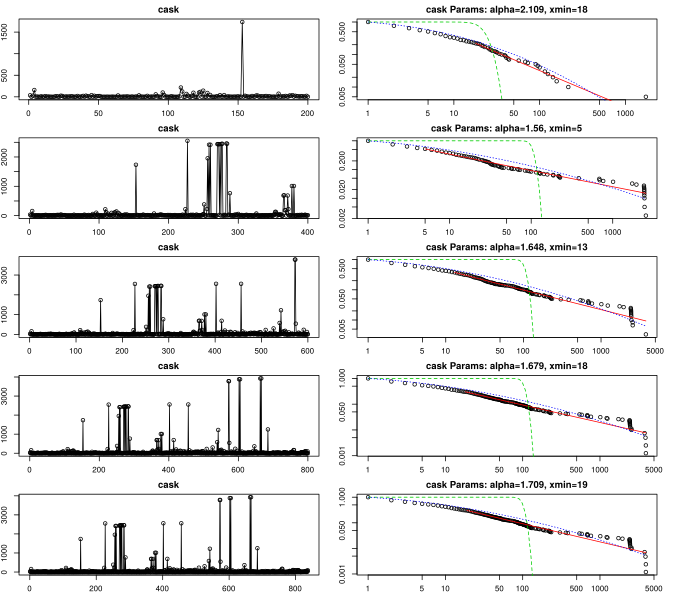
\includegraphics[width=0.95\textwidth]{img/adjusted_dist_cask.svg}}
	\caption{2-column plot fom cask repository. On the right side an simple plot with the number of lines changed in every commit in front of commit's number is presented. For this particular temporal segment we plot the PDF plot of it, presenting possible distributions fits: Red,power laws; Blue, Log Normal; Green: Poisson}
	\label{fig:cask}
      \end{figure*}

     
\begin{figure*}[htbp]
	\centerline{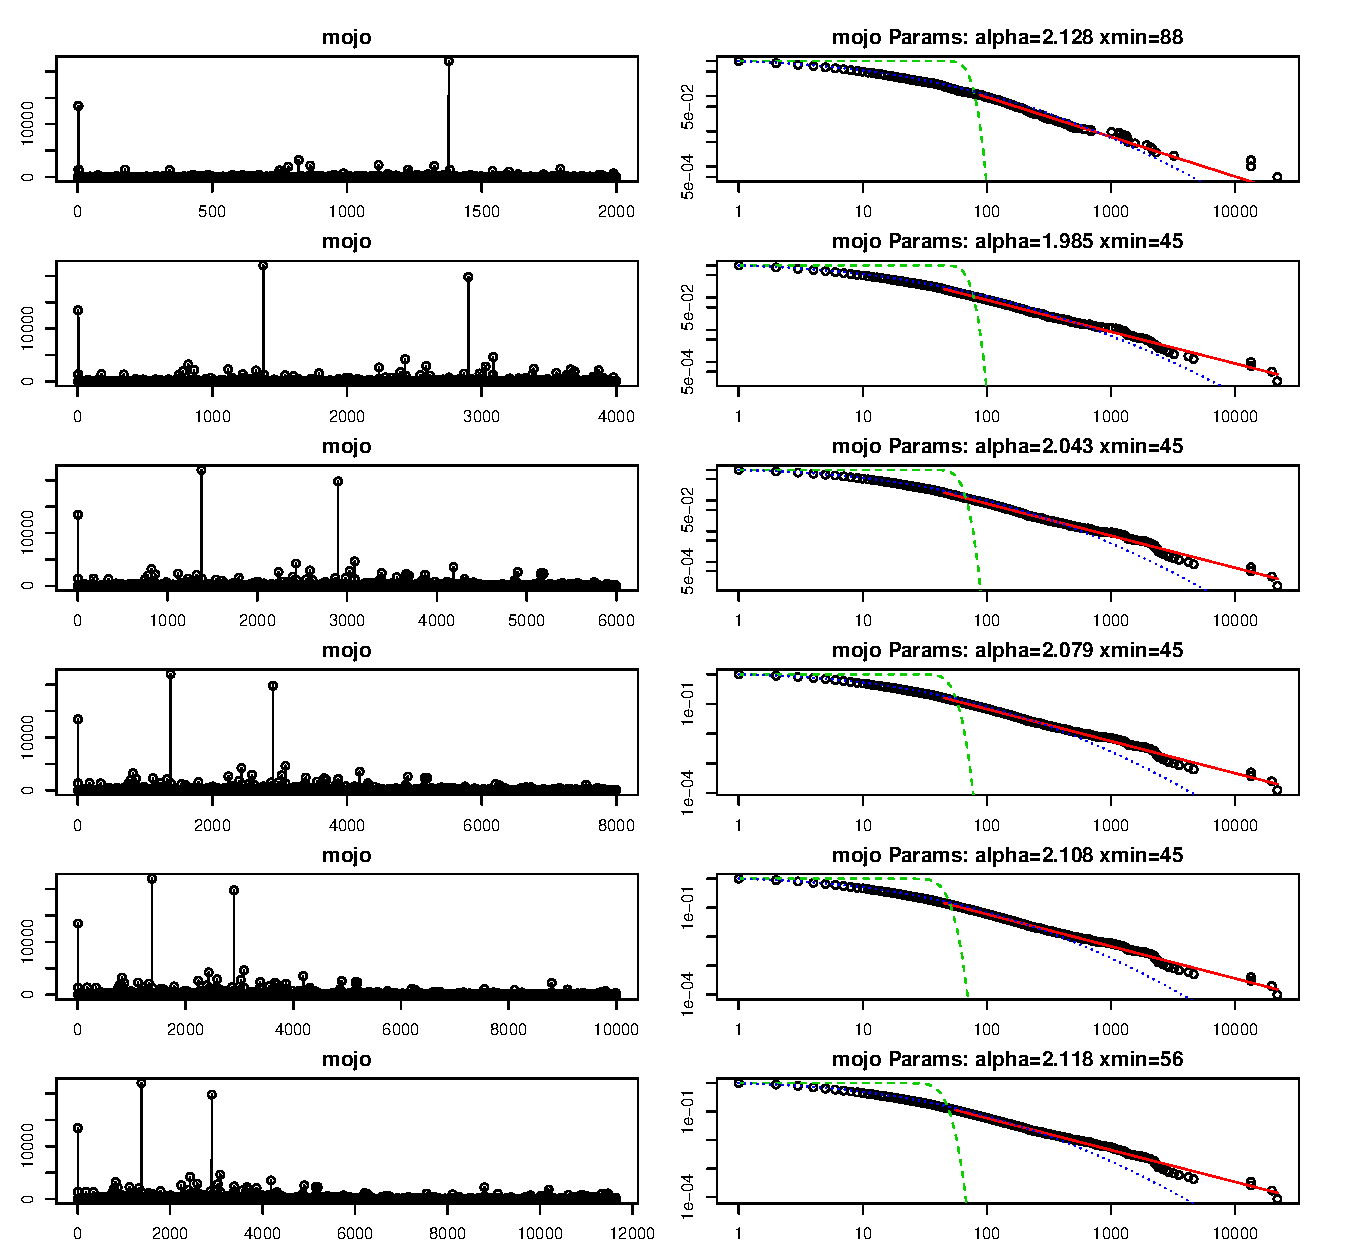
\includegraphics[width=0.95\textwidth]{img/mojo_global_estimation.eps}}
	\caption{2-column plot fom mojo repository. On the right side an simple plot with the number of lines changed in every commit in front of commit's number is presented. For this particular temporal segment we plot the PDF plot of it, presenting possible distributions fits: Red,power laws; Blue, Log Normal; Green: Poisson}
	\label{fig:mojo}
      \end{figure*}


\begin{figure*}[htbp]
	\centerline{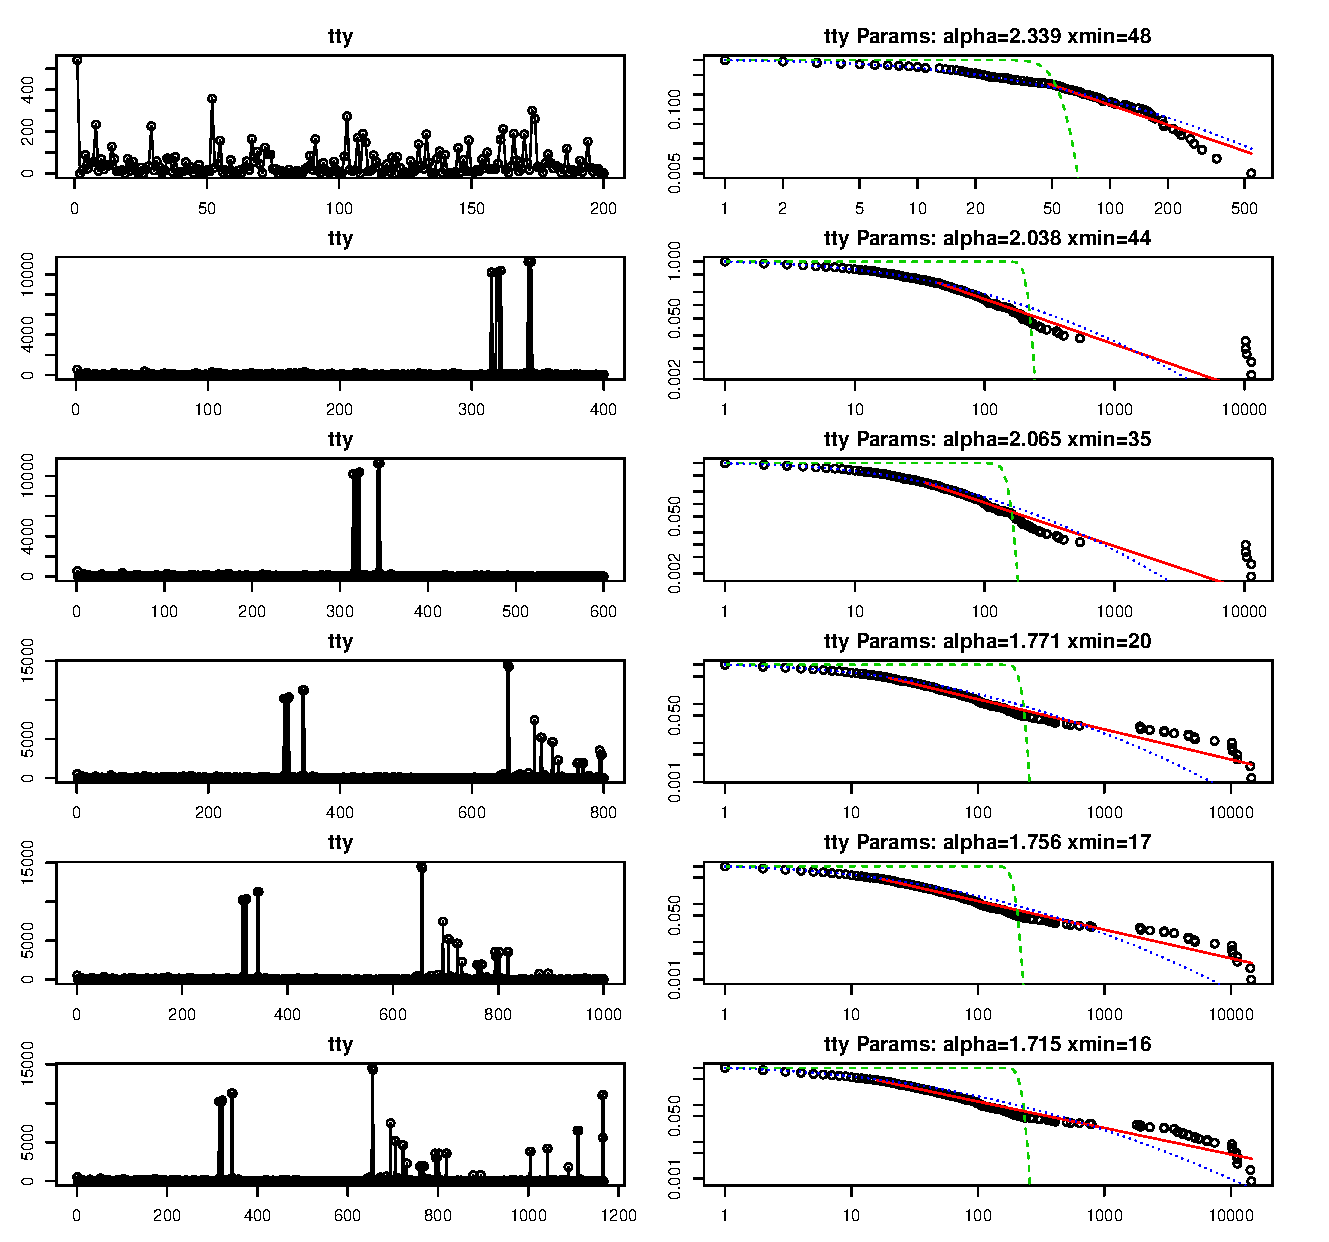
\includegraphics[width=0.95\textwidth]{img/tty_global.eps}}
	\caption{2-column plot fom tty repository. On the right side an simple plot with the number of lines changed in every commit in front of commit's number is presented. For this particular temporal segment we plot the PDF plot of it, presenting possible distributions fits: Red,power laws; Blue, Log Normal; Green: Poisson}
	\label{fig:tty}
\end{figure*}

\begin{figure*}[htbp]
	\centerline{\includegraphics[width=0.95\textwidth]{img/rakudo_global_plot.eps}}
	\caption{2-column plot fom rakudo repository. On the right side an simple plot with the number of lines changed in every commit in front of commit's number is presented. For this particular temporal segment we plot the PDF plot of it, presenting possible distributions fits: Red,power laws; Blue, Log Normal; Green: Poisson}
	\label{fig:rakudo}
\end{figure*}

\begin{figure*}[htbp]
	\centerline{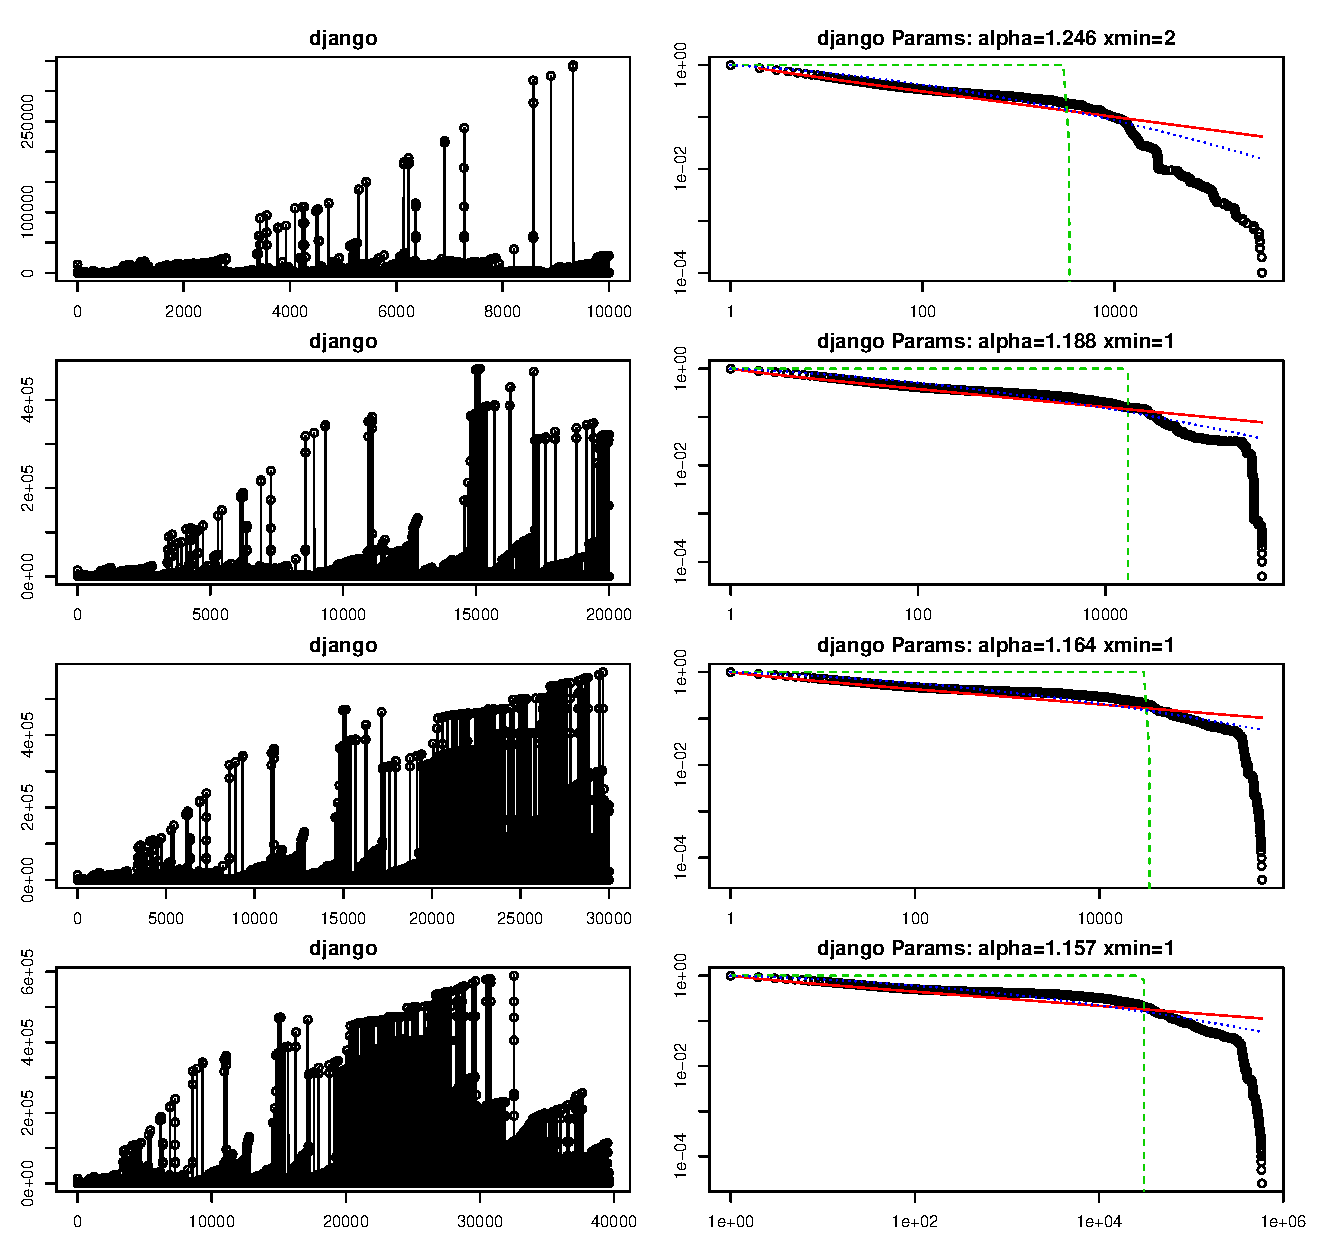
\includegraphics[width=0.95\textwidth]{img/django_global_set.eps}}
	\caption{2-column plot fom Django repository. On the right side an simple plot with the number of lines changed in every commit in front of commit's number is presented. For this particular temporal segment we plot the PDF plot of it, presenting possible distributions fits: Red,power laws; Blue, Log Normal; Green: Poisson }
	\label{fig:django}
\end{figure*}


\begin{table*}[h!tbp]
	\caption{Cask summary results}
	\begin{center}
		\begin{tabular}{| p{0.12\linewidth} | p{0.08\linewidth} | p{0.08\linewidth} | p{0.08\linewidth} | p{0.1\linewidth} |p{0.13\linewidth} | p{0.09\linewidth} |}
			\hline
                  Commit range & PL vs. LogN & PL vs. Exp & PL vs. PLtrunc & Result \\
                  Commit range 1 &  LogN & PL  & PL vs. PLtrunc & Result \\
                  Commit range 2& ND & PL  & ND & Result \\
                  Commit range 3& ND  &  PL & ND & Result \\
                  Commit range 4& ND & PL  & ND & Result \\
			\hline

			\hline
		\end{tabular}
	\end{center}
\label{tab:2019testscask}
\end{table*}

\begin{table*}[h!tbp]
	\caption{Django summary results}
	\begin{center}
		\begin{tabular}{| p{0.12\linewidth} | p{0.08\linewidth} | p{0.08\linewidth} | p{0.08\linewidth} | p{0.1\linewidth} |p{0.13\linewidth} | p{0.09\linewidth} |}
			\hline
                  Commit range & PL vs. LogN & PL vs. Exp & PL vs. PLtrunc & Result \\
                  Commit range 1 &  LogN & PL  &PLtrunc & Result \\
                  Commit range 2&  LogN & PL  &PLtrunc & Result \\
                  Commit range 3&  LogN & PL  &PLtrunc & Result \\
                  Commit range 4&  LogN & PL  &PLtrunc & Result \\
			\hline

			\hline
		\end{tabular}
	\end{center}
\label{tab:2019testsdjango}
\end{table*}


\begin{table*}[h!tbp]
	\caption{Rakudo summary results}
	\begin{center}
		\begin{tabular}{| p{0.12\linewidth} | p{0.08\linewidth} | p{0.08\linewidth} | p{0.08\linewidth} | p{0.1\linewidth} |p{0.13\linewidth} | p{0.09\linewidth} |}
			\hline
                  Commit range & PL vs. LogN & PL vs. Exp & PL vs. PLtrunc & Result \\
                  Commit range 1 &   LogN & PL  &PLtrunc & Result \\
                  Commit range 2&  LogN & PL  &PLtrunc & Result \\
                  Commit range 3&  LogN & PL  &PLtrunc & Result \\
                  Commit range 4&  LogN & PL  &PLtrunc & Result \\
			\hline

			\hline
		\end{tabular}
	\end{center}
\label{tab:2019testsrakudo}
\end{table*}


\begin{table*}[h!tbp]
	\caption{Mojo summary results}
	\begin{center}
		\begin{tabular}{| p{0.12\linewidth} | p{0.08\linewidth} | p{0.08\linewidth} | p{0.08\linewidth} | p{0.1\linewidth} |p{0.13\linewidth} | p{0.09\linewidth} |}
			\hline
                  Commit range & PL vs. LogN & PL vs. Exp & PL vs. PLtrunc & Result \\
                  Commit range 1 &  ND & PL  & ND & Result \\
                  Commit range 2& ND & PL  & ND & Result \\
                  Commit range 3& ND  &  PL & ND & Result \\
                  Commit range 4& ND & PL  & ND & Result \\
			\hline

			\hline
		\end{tabular}
	\end{center}
\label{tab:2019testsmojo}
\end{table*}


\begin{table*}[h!tbp]
	\caption{tty summary results}
	\begin{center}
		\begin{tabular}{| p{0.12\linewidth} | p{0.08\linewidth} | p{0.08\linewidth} | p{0.08\linewidth} | p{0.1\linewidth} |p{0.13\linewidth} | p{0.09\linewidth} |}
			\hline
                  Commit range & PL vs. LogN & PL vs. Exp & PL vs. PLtrunc & Result \\
                  Commit range 1 & ND & ND  & PLtrunc & Result \\
                  Commit range 2& ND & PL  & ND & Result \\
                  Commit range 3& ND  &  PL & ND & Result \\
                  Commit range 4& ND & PL  & ND & Result \\
			\hline

			\hline
		\end{tabular}
	\end{center}
\label{tab:2019teststty}
\end{table*}


% --------------------------------------------------------


\section{Conclusions}\label{conc}


\bibliographystyle{apalike} \bibliography{biblio}

\end{document}
